\documentclass{beamer}
\usepackage[utf8x]{inputenc}
\usepackage{listings}
\usepackage{hyperref}
\usepackage{graphicx}
\usepackage{tabularx}
\lstset{language=C}
\usepackage{calc}
\usepackage[export]{adjustbox}
\usepackage{lineno}


\title{\textbf{PROGETTO DI INGEGNERIA DI INTERNET E DEL WEB}}
\subtitle{Web Server con Adattamento Dinamico di Contenuti Statici}
\author{Giulia Cassarà \\ 
 \medskip
Giorgio Iannone
\medskip
\\ Emanuele Savo
}
\date{19 Settembre 2017}
\setbeamertemplate{navigation symbols}{}


\begin{document}
\begin{frame}
\centerline{\includegraphics[height=30mm]{/home/giorgio/Scrivania/RelazioneIIW/miaParte/torvergata.png}\hspace{2em}}
\maketitle


\end{frame}


\begin{frame}
\frametitle{Introduzione}
\framesubtitle{Hideo}
\begin{figure}
	\includegraphics[width=.1\textwidth,right]{/home/giorgio/Scrivania/RelazioneIIW/miaParte/favicon.png}
\end{figure}

Il progetto \textbf{Hideo} è un web server con supporto minimale del protocollo
HTTP/1.1 realizzato in linguaggio C usando le API della socket Berkeley.

\medskip

Il suo scopo è offrire agli utenti la possibilità di scaricare immagini adattandole alle caratteristiche ed alle necessità del
dispositivo richiedente.

\footnotesize
\begin{itemize}
\item Quando un client si connette viene reindirizzato sulla pagina principale in cui sono presenti le miniature delle immagini disponibili per il
download.
\item Cliccando su un’immagine, essa viene convertita automaticamente dal
server e poi consegnata all’utente nella risoluzione e qualità ottimale per il suo
device.
\item L’immagine convertita viene poi salvata dal server in una cache,
risparmiando il carico di lavoro e diminuendo i tempi di risposta in caso di
successive richieste.
\end{itemize}
\normalsize
\end{frame}


\begin{frame}
\frametitle{Introduzione}
\framesubtitle{Hideo}
Il web server ha un’architettura \textbf{multithread} con pool di thread statico, quindi è
capace di gestire più connessioni simultaneamente ed adotta un sistema di logging
basato su livelli per discriminare i vari tipi di messaggi: \textit{information, warning,
error}.


\medskip

Il codice sorgente è disponibile al seguente indirizzo:

\medskip

\setlength{\parindent}{32pt} \href{https://github.com/v2-dev/hideo}{\color{blue}  https://github.com/v2-dev/hideo}


\end{frame}

\begin{frame}
\frametitle{Comportamento dell'applicazione}
\framesubtitle{Inizializzazione}

All'avvio del programma viene eseguita
la lettura ed il parsing del file di configurazione \textit{server.cfg}, contenente i seguenti parametri:

\begin{itemize}
\item porta di ascolto
\item numero di thread
\item lunghezza del backlog
\item livello di logging
\end{itemize}


L’eseguibile inizializza la socket d’ascolto e le strutture dati
relative al modulo WURFL (caricamento del database di \textit{User Agent}), alla cache ed al logger con i parametri scelti.

\end{frame}


\begin{frame}
\frametitle{Comportamento dell'applicazione}
\framesubtitle{Multithreading}

Terminata l’inizializzazione, vengono spawnati i \textit{worker thread} che
si occupano di servire i client. L’eseguibile entra in un loop non terminante nel
quale:

\begin{itemize}
\item Accetta le connessioni dalla socket d’ascolto.
\item Accoda il file descriptor ad una lista FIFO acceduta in lettura dai worker thread in stato
di IDLE.
\item Ai thread viene segnalato l'inserimento di nuovo file descriptor alla lista, e mediante l’utilizzo di un \textbf{mutex} uno dei thread
prende l’esclusività su tale socket,
rimuovendola dalla lista e servendo il client ivi collegato mantenendo aperta e
sfruttando tale socket (permanenza della connessione del protocollo HTTP/1.1).
\end{itemize}

\end{frame}


\begin{frame}
\frametitle{Comportamento dell'applicazione}
\framesubtitle{Processamento della richiesta}

Il thread, terminata la copiatura della socket ad un buffer interno, effettua un
parsing del messaggio per:

\begin{itemize}
\item Controllarne l’effettiva validità ed aderenza alle
specifiche HTTP/1.1

\item per discriminare tra i metodi \textbf{GET} ed \textbf{HEAD} (di cui
veniva richiesta l’implementazione).
\end{itemize}

\end{frame}

\begin{frame}
\frametitle{Comportamento dell'applicazione}
\framesubtitle{Processamento della richiesta}

\begin{itemize}

\item Si ottiene dal modulo WURFL la risoluzione del
dispositivo richiedente, e vengono memorizzati il percorso del file richiesto
ed i parametri specificati nel campo HTTP \textit{Accept} quali il fattore di qualità e
l’estensione richiesta per l’immagine.

\item Nel caso la richiesta riguardi un’immagine interviene il modulo cacher, che si
occupa di inoltrare immediatamente il file se questi è presente in cache, senza
dover così eseguire nuovamente alcuna operazione di conversione.

\item In caso di
fallimento
della
ricerca
l’immagine
viene
convertita
dal
programma
\textbf{ImageMagick}, inviata al client e salvata nella cache.
\end{itemize}
\end{frame}



\begin{frame}
\frametitle{Comportamento dell'applicazione}
\framesubtitle{Inoltro del contenuto \& Chiusura della connessione}
\begin{itemize}
\item Una volta intervenuto il cacher (nel caso delle immagini) od appurato che non vi
siano errori di apertura della \textit{index.html} l’applicativo si occupa di inoltrare una
risposta al client, allegando o meno il file richiesto.

\item In caso di errori con il file
richiesto viene inoltrato un messaggio di errore \textbf{HTTP 404} mentre, nel caso di un
metodo non implementato, l’errore \textbf{501}.

\item La connessione verrà chiusa all’esplicita disconnessione del client od, in sua
assenza, allo scadere di un timeout di connessione altrimenti resettato ad ogni
nuova richiesta.
\end{itemize}
\end{frame}








\begin{frame}
\frametitle{WURFL}
\framesubtitle{Introduzione}

\begin{figure}
    \includegraphics[width=.3\textwidth,right]{/home/giorgio/Scrivania/RelazioneIIW/miaParte/wurfl.png}
\end{figure}

\textbf{WURFL} è un \textit{DDR} (Device Description Repository) sviluppato da \textbf{ScientiaMobile}, ed è composto da un set di \textbf{API} e librerie che permettono di consultare il proprio database e fornire, dato in input lo \textit{User Agent}, il maggior
numero di informazioni sul dispositivo che sta navigando su un sito web.

\begin{itemize}
\item Nel nostro caso abbiamo sfruttato le API di WURFL per ottenere i valori di risoluzione dei dispositivi
\item Per ottenere una Trial di WURFL bisogna fare richiesta su \href{https://www.scientiamobile.com/}{\color{blue}  https://www.scientiamobile.com/}
\item Documentazione ufficiale: \href{https://docs.scientiamobile.com/documentation/infuze/infuze-c-api-user-guide}{\color{blue}  https://docs.scientiamobile.com/documentation/infuze/infuze-c-api-user-guide}

\end{itemize}
\end{frame}

\begin{frame}
\frametitle{WURFL}
\framesubtitle{Funzionamento \& Multithreading}

Il funzionamento di \textbf{WURFL} consiste nel caricamento in memoria del database del programma (un file \textit{.xml} rappresentato in C da una variabile opaca \textit{wurfl\_handle}) ed alla sua
interrogazione riguardo i vari \textit{User Agent}.

\medskip

Dalla documentazione ufficiale si legge che:

\medskip

\textit{ ``WURFL engine is thread safe and the intended design is that multiple
threads share the same wurfl\_handle.''}

\begin{itemize}
\item Quindi \texttt{wurfl\_handle} è progettato per rispondere ad interrogazioni da più thread.
\item Essendo il nostro Web Server \textbf{multi-thread}, questo ci ha permesso di non gestire  il problema delle interrogazioni parallele.
\end{itemize}


\end{frame}
\begin{frame}

\frametitle{WURFL}
\framesubtitle{Limitazioni Wurfl}

\begin{itemize}

\item Il database di \textbf{WURFL} fornitoci è limitato e non aggiornato, contiene per lo più informazioni di User Agent di dispositivi mobili.
\item Per effettuare correttamente i test sull'adattamento dinamico delle immagini del nostro Web Server abbiamo utilizzato un addon per Firefox: \href{https://addons.mozilla.org/it/firefox/addon/user-agent-switcher/}{\color{blue}  https://addons.mozilla.org/it/firefox/addon/user-agent-switcher/}
\item \textbf{User Agent Switcher} permette di cambiare temporaneamente l'User Agent del browser con uno compatibile con il database di WURFL.

\end{itemize}



\end{frame}
\begin{frame}
\frametitle{WURFL}
\framesubtitle{Samsung Galaxy Grand Neo 800x400}


\includegraphics[width=10cm,height=10cm,keepaspectratio]{/home/giorgio/Scrivania/RelazioneIIW/miaParte/GrandNeo.png}



\end{frame}

\begin{frame}
\frametitle{WURFL}
\framesubtitle{Samsung Galaxy S5 1920x1080}


\includegraphics[width=10cm,height=10cm,keepaspectratio]{/home/giorgio/Scrivania/RelazioneIIW/miaParte/S5.png}



\end{frame}


\begin{frame}
\frametitle{WURFL}
\framesubtitle{Samsung Galaxy Tab Pro 2560x1600}


\includegraphics[width=10cm,height=10cm,keepaspectratio]{/home/giorgio/Scrivania/RelazioneIIW/miaParte/TabPro.png}



\end{frame}



\begin{frame}
\frametitle{Adattamento dell'Immagine}
\framesubtitle{ImageMagick}
\begin{figure}
    \includegraphics[width=.2\textwidth,right]{/home/giorgio/Scrivania/RelazioneIIW/miaParte/magick.png}
\end{figure}

Per convertire le immagini abbiamo utilizzato il comando \texttt{convert} della suite di manipolazione delle immagini \textbf{ImageMagick}.
\begin{itemize}
\item Link: \href{https://www.imagemagick.org/script/convert.php}{\color{blue}  https://www.imagemagick.org/script/convert.php} 
\item Il comando viene lanciato mediante la chiamata di sistema \texttt{system}, che è essenzialmente una \texttt{fork+execve+wait}.
\item Il thread che sta servendo il client crea quindi un processo figlio per eseguire il comando specificato, e rimane bloccato \textit{in attesa} che il figlio termini il suo lavoro, ovvero attende che la conversione dell'immagine sia completata.
\end{itemize}
\end{frame}



\begin{frame}
\frametitle{Adattamento dell'Immagine}
\framesubtitle{Osservazioni}

\textbf{Vantaggi:} 
\begin{itemize}
\item le conversioni non sono a carico \textit{diretto} del processo server, ma di processi creati \textit{ad hoc}.
\item implementazione relativamente facile.
\end{itemize}


\medskip

\textbf{Svantaggi:} 
\begin{itemize}
\item il thread deve comunque aspettare che la conversione \textit{i-esima} sia completata, prima di poter lanciare un nuovo processo per la conversione \textit{i+1-esima}.

\end{itemize}
\end{frame}

\begin{frame}
\frametitle{Adattamento dell'Immagine}
\framesubtitle{Un diverso approccio}

Abbiamo anche pensato ad \textbf{approcci migliori} che, tuttavia, abbiamo poi
\textit{abbandonato} per mantenere un codice più semplice e facile da debuggare. L'approccio alternativo consisteva nei seguenti passi:

\begin{itemize}
\item Il thread che serve il client legge la prima richiesta, e fa partire la prima conversione.
\item Senza aspettare che la conversione termini, legge la seconda richiesta, e fa partire la
seconda conversione, e così via.
\item Tra una lettura di una richiesta e l'altra, il thread \textit{controlla} quali sono le immagini che
sono state convertite completamente (ovvero i processi figli che hanno terminato il
proprio lavoro) ed \textit{evade} le relative richieste.
\
\end{itemize}

\end{frame}

\begin{frame}
\frametitle{Adattamento dell'Immagine}
\framesubtitle{Un diverso approccio}

\begin{itemize}
\item Una singola conversione \textit{non} blocca il thread, che risulterebbe così decisamente più
veloce nel servire le richiese del client.
\item Per creare il processo per la conversione anziché la chiamata system venivano
utilizzate \texttt{fork + execve}.
\item Per controllare se un processo è terminato basta eseguire la \texttt{waitpid} con parametro
\texttt{WNOHANG} (per rendere la verifica non bloccante).

\medskip

La \textbf{complessità} di questo approccio sta nel fatto che il thread deve \textit{ricordarsi} della storia passata, ovvero delle richieste ricevute ma non ancora evase.
\end{itemize}
\end{frame}



\begin{frame}
\frametitle{Struttura e Architettura dell'Applicazione}
\framesubtitle{Server}

Il Server è organizzato in due componenti principali:
\begin{itemize}
\item Una funzione main che si occupa della gestione della socket TCP
accettando nuove connessioni;
\item Un pool statico di thread worker che si occupa della gestione di ogni
singola connessione;
\end{itemize}


Il server è \textbf{prethreaded} con  un numero di thread statico fissato nel file di configurazione.


\medskip
\end{frame}

\begin{frame}
\frametitle{Struttura e Architettura dell'Applicazione}
\framesubtitle{Server Main}
La funzione \textbf{main} del server svolge i seguenti compiti:

\medskip

\begin{itemize}
\item Inizializzazione delle componenti Cacher, Logger, WURFL.
\item Inizializzazione e gestione della socket TCP sulla porta specificata nel file di configurazione.
\item Il main entra in un ciclo in cui accetta continuamente richieste di connessione in entrata, salvando la relativa connessione in una lista chiamata \textit{list\_sock} e \textit{sveglia} mediante una \texttt{signal} uno dei thread del pool in attesa sulla \texttt{condition}.
\end{itemize}

\end{frame}



\begin{frame}
\frametitle{Struttura e Architettura dell'Applicazione}
\framesubtitle{Thread job}

\begin{itemize}
\item Ogni thread del pool esegue la funzione \texttt{thread\_main}.
\item Se non vuota, il worker
estrae una socket dalla lista \texttt{list\_sock}, altrimenti si mette in attesa di una nuova
\texttt{signal} dal thread main.
\item   Il thread che è stato risvegliato chiama la funzione
\texttt{thread\_job()} in cui serve in loop il client connesso alla socket:
\end{itemize}

\medskip
\scriptsize
\setlength{\parindent}{30pt} \textit{infinite loop}

\setlength{\parindent}{32pt} \textit{\{}

\setlength{\parindent}{50pt} \textit{serve\_request(socket\_client);}

\setlength{\parindent}{50pt} \textit{if (some\_error)}

\setlength{\parindent}{52pt} \textit{\{}


\setlength{\parindent}{70pt} \textit{free(socket\_client);}

\setlength{\parindent}{70pt} \textit{close(socket\_client);}

\setlength{\parindent}{70pt} \textit{break loop;}


\setlength{\parindent}{52pt} \textit{\}}

\setlength{\parindent}{50pt} \textit{else}


\setlength{\parindent}{70pt} \textit{continue loop serving client;}

\setlength{\parindent}{32pt} \textit{\}}
\normalsize
\end{frame}

\begin{frame}
\frametitle{Struttura e Architettura dell'Applicazione}
\framesubtitle{Funzione serve\_request}

Nella funzione \texttt{serve\_request(socket\_client)} viene effettuato il parsing della richiesta HTTP:

\begin{itemize}
\item Viene fatto il parsing del metodo, accettando esclusivamente richieste \textbf{GET} o \textbf{HEAD}.
\item Viene fatto il parsing del path richiesto, verificando l'assenza di errori.
\item Viene fatto il parsing dei campi HTTP e vengono posti in buffer, se presenti, i campi \textit{Accept} ed \textit{User Agent}.
\item Se gli header sono corretti, viene passato lo User Agent al modulo
\textbf{WURFL} per ricavare
valori di altezza e larghezza ottimali per lo User-Agent ricevuto.
\end{itemize}

\end{frame}


\begin{frame}
\frametitle{Struttura e Architettura dell'Applicazione}
\framesubtitle{Funzione serve\_request}


\begin{itemize}
\item Il thread controlla la presenza di parametri riguardanti l’estensione ed il
fattore di qualità del contenuto richiesto presenti nel campo \textit{Accept}.
\begin{itemize}
\item Se il client non specifica alcun campo
Accept (o specifica un generico Accept: */*) vengono assunti come
valori di default il formato PNG ed un fattore di qualità q = 1.0.
\end{itemize}
\item Si richiede l'immagine alla cache
richiamando la funzione \texttt{obtain\_file(params)} specificando nome,
risoluzione, fattore di qualità ed estensione del file richiesta.
\item Se l’immagine richiesta non è presente in cache essa viene convertita
chiamando la funzione esterna \texttt{nConvert} di ImageMagick. Dopo la conversione il file viene
aggiunto nella cache e inviato al client.
\end{itemize}

\end{frame}










\begin{frame}
\frametitle{Cache}
\framesubtitle{Introduzione}

\begin{itemize}
\item Cache di tipo \textbf{LRU} (Least Recently Used).
\item La cache memorizza in memoria secondaria tutti i file
convertiti, senza cancellarli e mantiene in RAM i file utilizzati più di recente, in
modo da poterli servire più velocemente ai thread che ne fanno richiesta.
\end{itemize}



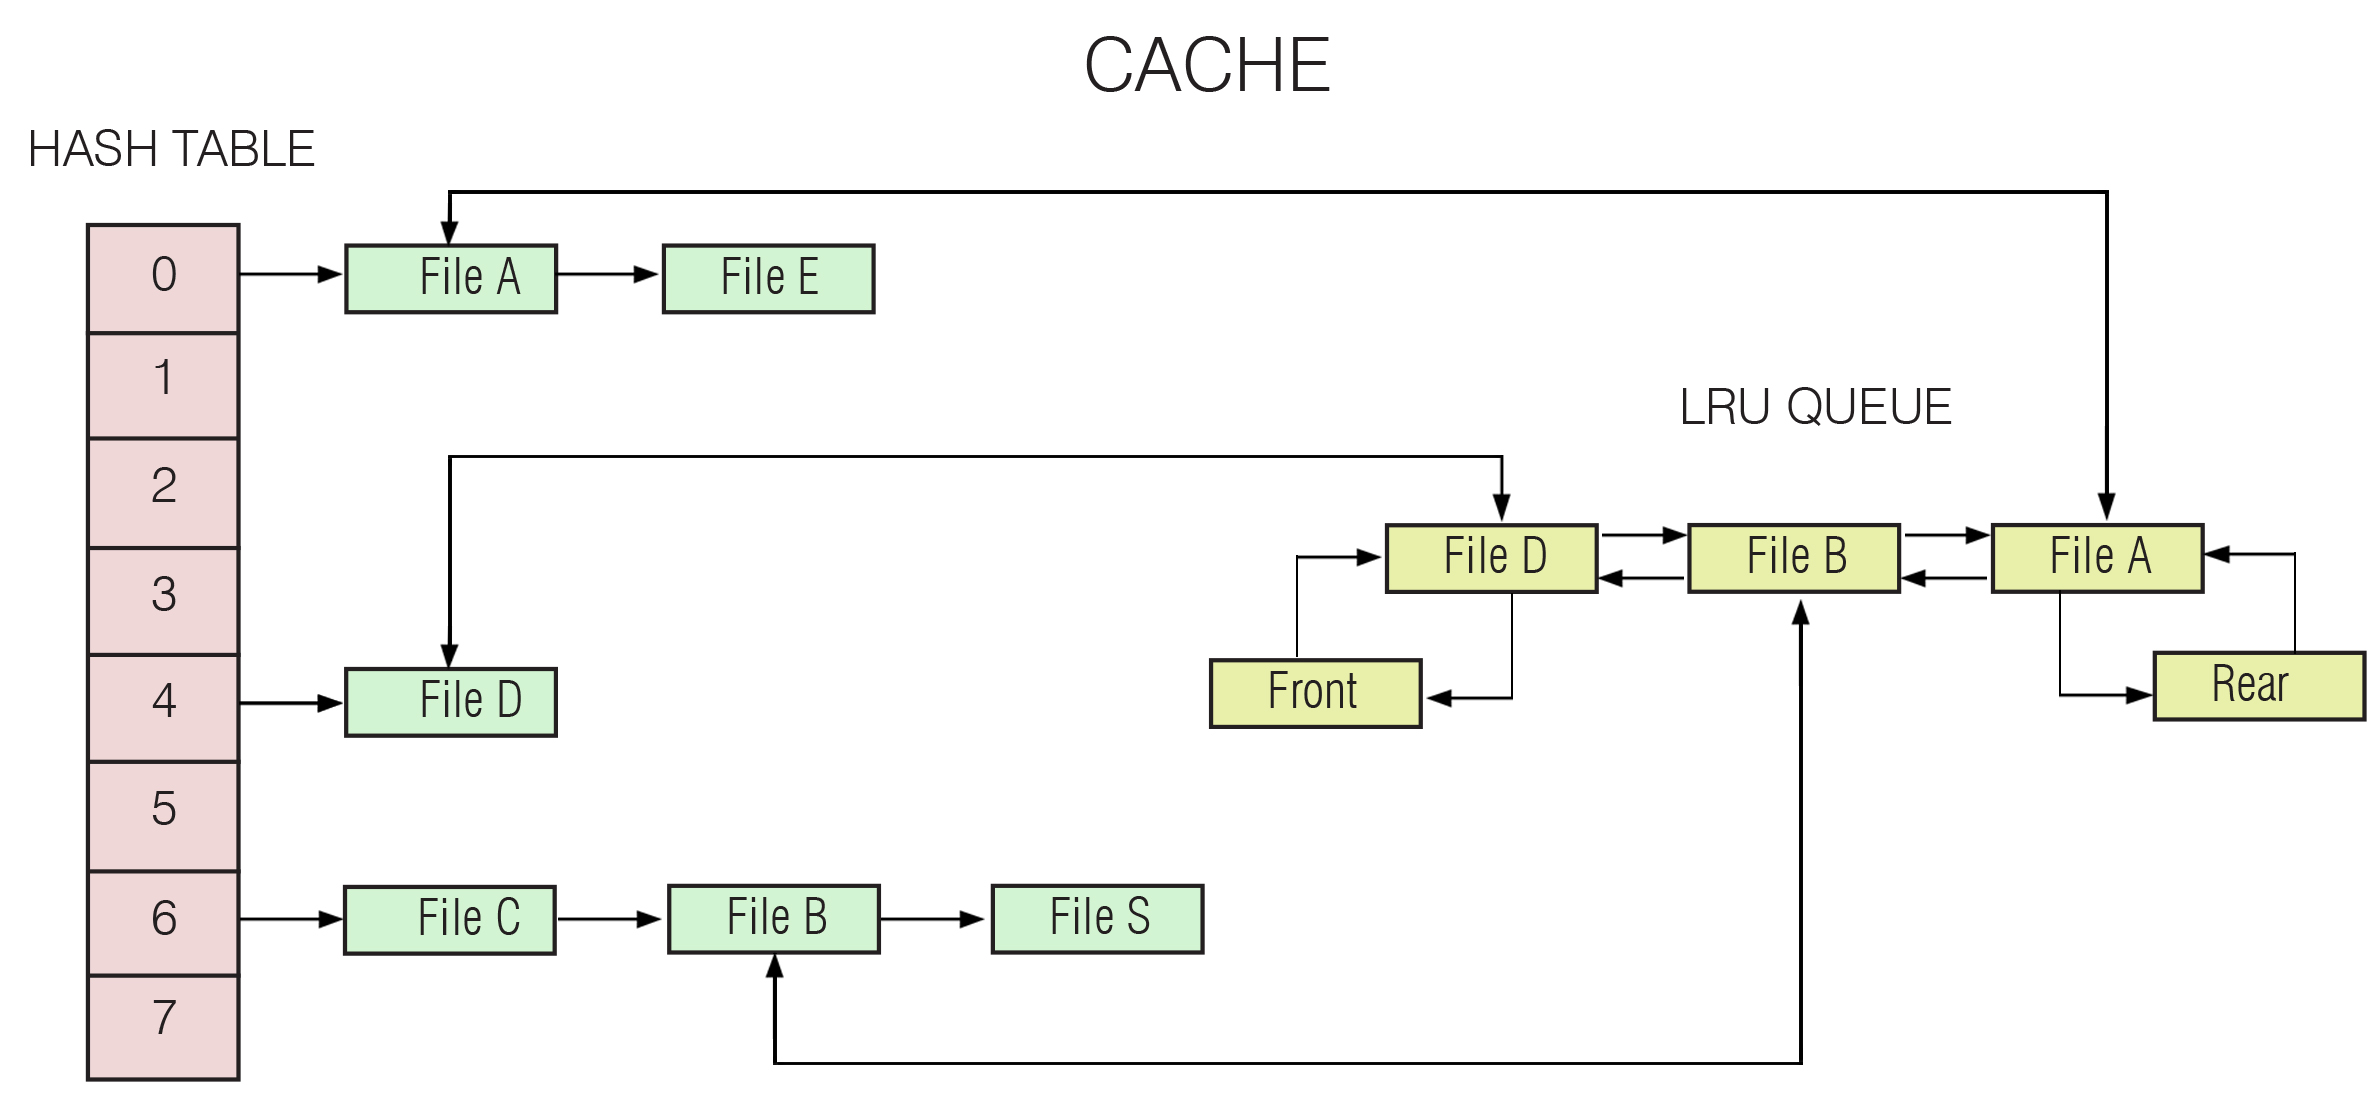
\includegraphics[width=10cm,height=10cm,keepaspectratio]{/home/giorgio/Scrivania/RelazioneIIW/miaParte/cache.jpg}

\end{frame}



\begin{frame}
\frametitle{Cache}
\framesubtitle{Strutture dati}
\begin{itemize}
\item \textbf{Tabella hash con liste di collisione:}
\begin{itemize}
\item Una tabella contenente entry chiamate \textit{hashNode}.
\item Un \textit{hashNode} rappresenta un file presente su disco, contenendo informazioni
sul file quali il percorso completo.
\item Un file rappresentato da un \textit{hashNode} non necessariamente è presente anche
in RAM.
\end{itemize}
\end{itemize}



\begin{itemize}
\item \textbf{Coda LRU:}
\begin{itemize}
\item Una coda che memorizza entry chiamate \textit{ramNode}.
\item Un \textit{ramNode} rappresenta un file caricato in RAM.
\item Un \textit{ramNode} contiene l'indirizzo del file caricato in RAM (tramite mmap)
\item I \textit{ramNode} utilizzati più recentemente vengono “spinti” verso la testa, quelli
meno utilizzati recentemente rimangono accodati.
\end{itemize}
\end{itemize}
\end{frame}
\begin{frame}
\frametitle{Cache}
\framesubtitle{Inserimento iniziale di una entry}

L'inserimento iniziale di un' immagine nella cache consiste nel:


\begin{itemize}
\item Eseguire la conversione del file originale con i parametri specificati.
\item Salvare il file convertito nella cartella cache, secondo lo schema: \textit{“./cache/fileA/x/y/q/fileA.jpg"}.

\item Una volta terminata la conversione viene creato l'\textit{hashNode} ed inserito nella
tabella hash.
\item Viene infine creato il \textit{ramNode}, che viene inserito in testa della coda LRU.
\end{itemize}
\end{frame}

\begin{frame}
\frametitle{Cache}
\framesubtitle{Richiesta di un file}

Supponiamo di richiedere un file \textit{A} al gestore della cache:
\medskip

Il gestore esegue una ricerca nella tabella hash per vedere innanzitutto se il file
\textit{A} è presente su disco:

\begin{itemize}
\item Se non esiste l'\textit{hashNode} relativo al file \textit{A}, significa che non esiste quel file
su disco, perciò si esegue l' \textbf{inserimento iniziale di una entry}.
\item Se la ricerca ha successo significa che il gestore ha trovato l'\textit{hashNode}
relativo al file \textit{A}, quindi certamente il file \textit{A} è presente su disco.
\end{itemize}


\end{frame}

\begin{frame}
\frametitle{Cache}
\framesubtitle{Richiesta di un file}
Se l’\textit{hashNode} è stato trovato, si valuta il contenuto del suo puntatore al \textit{ramNode}:

\begin{itemize}
\item Se questo campo è diverso da NULL, allora il file \textit{A} è anche caricato in
RAM:
\begin{itemize}
\item Il gestore ottiene immediatamente il \textit{ramNode} del file \textit{A}.
\item Sposta il \textit{ramNode} del file \textit{A} in testa alla coda LRU, in quanto ultimo file
richiesto.
\item Restituisce l'indirizzo in RAM del file.
\end{itemize}
\item Se invece il campo puntatore è uguale a NULL, vuole dire che il file \textit{A} non è
caricato in RAM:
\begin{itemize}
\item Bisogna fare la \texttt{open} del file mediante il nome completo indicato.
\item Eseguire una \texttt{mmap} del file descriptor ottenuto.
\item Inizializzare un nuovo \textit{ramNode} con i giusti parametri.
\item Inserire il \textit{ramNode} alla testa della coda LRU.
\item Restituire al thread l’indirizzo del mapping.
\end{itemize}
\end{itemize}

\end{frame}


\begin{frame}
\frametitle{Cache}
\framesubtitle{Richiesta di un file}

\begin{center}
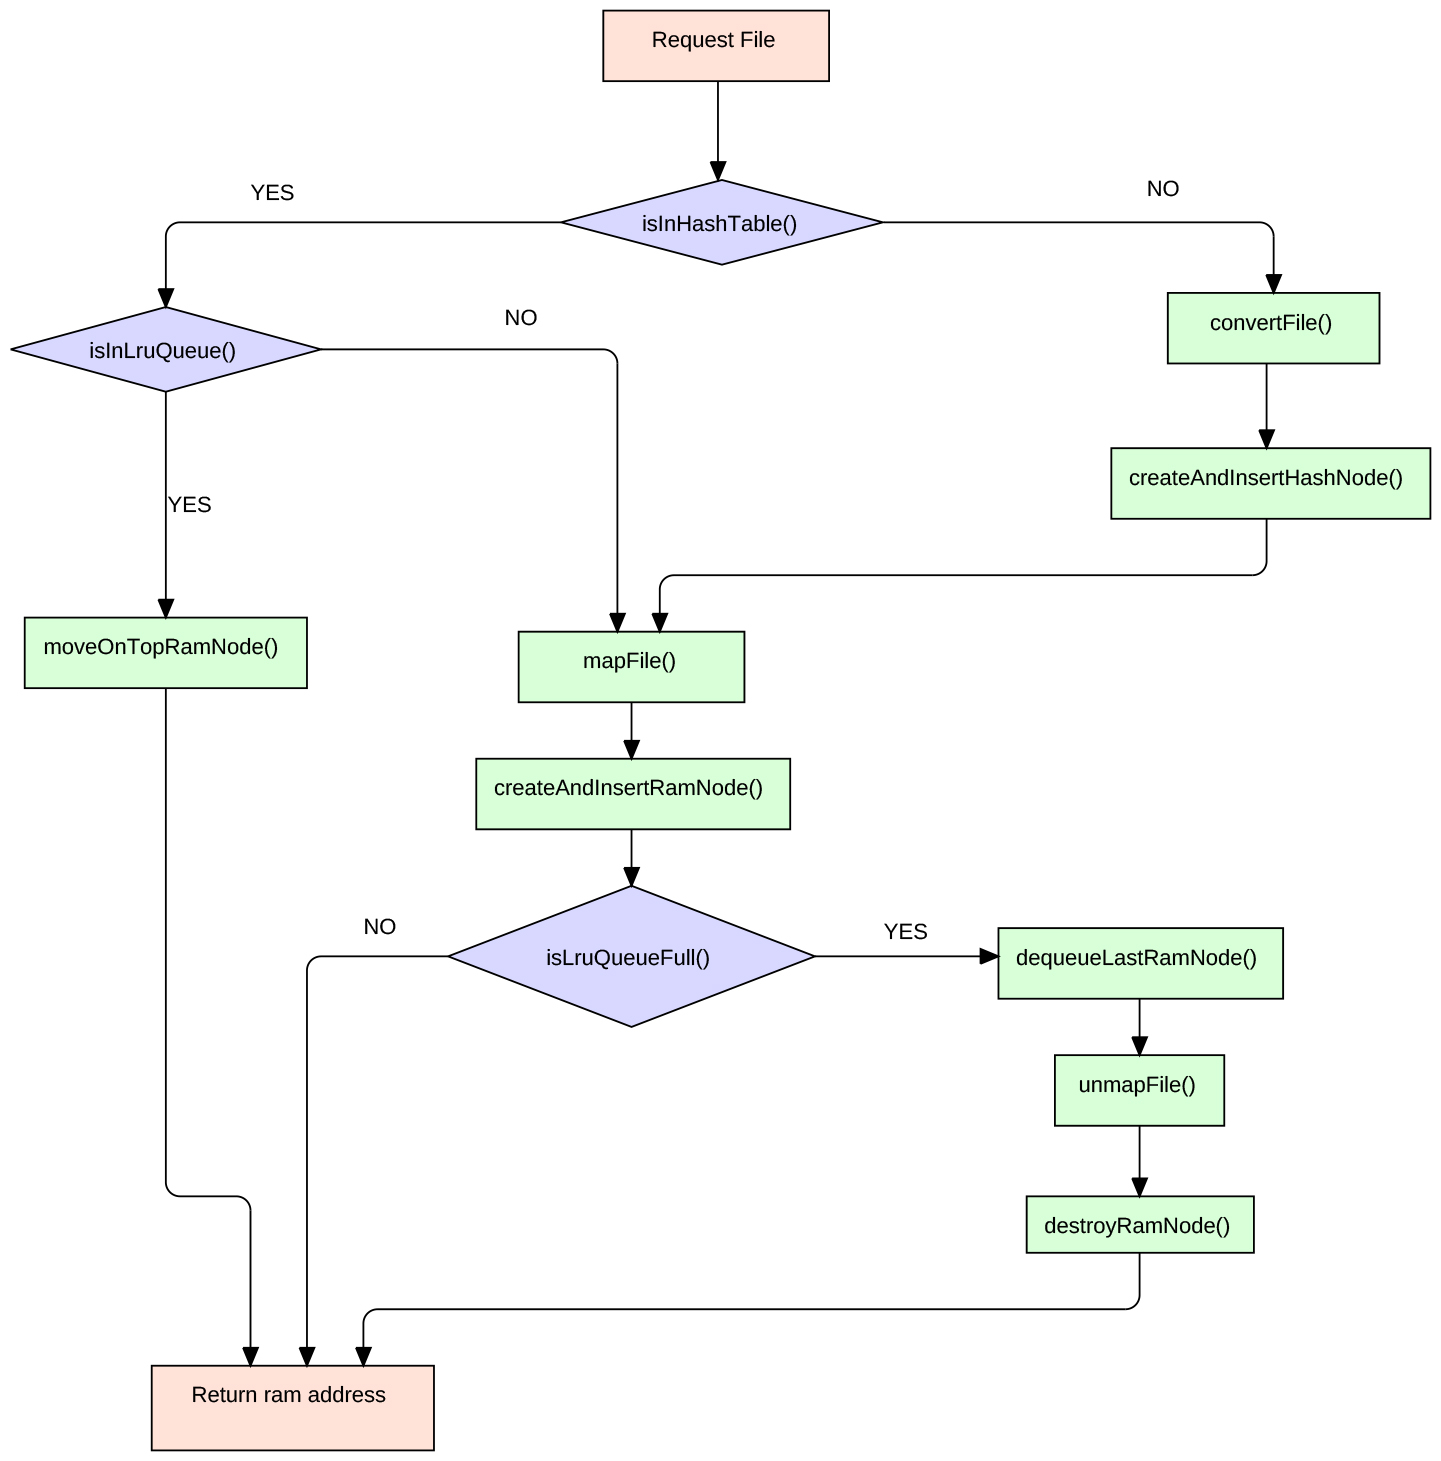
\includegraphics[width=12cm,height=8cm,keepaspectratio]{/home/giorgio/Scrivania/RelazioneIIW/miaParte/cache2.jpg}
\end{center}


\end{frame}


\begin{frame}
\frametitle{Cache}
\framesubtitle{Osservazioni}


L’implementazione della cache poteva \textit{limitarsi} alla sola coda LRU, tuttavia
l’aggiunta di una tabella hash per i file non caricati in memoria ha apportato
notevoli vantaggi:
\begin{itemize}
\item Essendo una struttura dati memorizzata in RAM ci permette di sapere in tempi
rapidi quali file sono memorizzati su disco, evitando ad ogni richiesta una
\texttt{open}, che \textit{rappresenterebbe} un collo di bottiglia nelle prestazioni generali del server.
\item La tabella hash ci informa dell’eventuale presenza di tale file in RAM, \textit{evitando}
una scansione della coda LRU.
\end{itemize}
\end{frame}


\begin{frame}
\frametitle{Cache}
\framesubtitle{Prestazioni}

\textbf{Inserimento hashNode:}
L'inserimento di un \textit{hashNode} nella tabella hash consiste nel trovare la lista
di collisione a lui `` prefissata``  mediante la funzione hash sul nome del file,
presentando quindi un costo $O(1)$.

\medskip

\textbf{Inserimento ramNode:}
Anche l’inserimento di un \textit{ramNode} ha costo $O(1$), in quanto consiste
nella modifica di puntatori nella testa della coda.

\medskip

\textbf{Cancellazione hashNode:} Gli \textit{hashNode} non vengono mai cancellati.
\end{frame}
\begin{frame}
\frametitle{Cache}
\framesubtitle{Prestazioni}

\textbf{Cancellazione ramNode:} Vengono cancellati solo i \textit{ramNode}
che si trovano in fondo alla coda LRU:

\begin{itemize}


\item Per trovare questi nodi è sufficiente
accedere al nodo ``Rear''  della coda LRU e vedere all'indietro a quale
\textit{ramNode} punta.

\medskip

\item Una volta eliminato il \textit{ramNode} bisogna notificare all'\textit{hashNode} associato
che il suo \textit{ramNode} non esiste più, bisogna cioè modificare il campo
puntatore dell'\textit{hashNode} che punta al \textit{ramNode}, settandolo al valore
\texttt{NULL}.

\medskip

\item Grazie ad un puntatore
gemello che collega il \textit{ramNode} all'\textit{hashNode} associato troviamo immediatamente l'\textit{hashNode} che ci
interessa. Di conseguenza, anche la cancellazione presenta un costo
costante $O(1)$.


\end{itemize}

\end{frame}

\begin{frame}
\frametitle{Cache}
\framesubtitle{Prestazioni}
\textbf{Ricerca ramNode:} il costo per la ricerca del \textit{ramNode} è dato dal costo della ricerca
dell'\textit{hashNode}, infatti una volta trovato l'\textit{hashNode} recuperiamo
immediatamente il \textit{ramNode} associato, accedendo semplicemente al
campo puntatore. Il costo per la ricerca di un \textit{hashNode} è dato da:

\begin{center}
$T_{avg}(n) = O(1+\alpha)$, con $\alpha = n/m$
\end{center}


dove:

\medskip

$n$: numero di \textit{hashNode} presenti nella tabella hash

$m$: numero di liste di collisione della tabella

\medskip

Se il fattore di carico $\alpha$ si mantiene ``stabile'' (numero di collisioni) il tempo di ricerca può essere considerato
pari ad un costo costante $O(1)$.

\end{frame}

\begin{frame}[fragile]
\frametitle{Cache}
\framesubtitle{Interfacce utilizzate}

\tiny
\begin{lstlisting}
char * obtain_file(struct cache * web_cache, char * name,
	char * ext, int x, int y, int q, int * size, int file_type);
	
	
void release_file(struct cache * myCache, char * name, char * ext,
	int x, int y, int q, int file_type);
	
\end{lstlisting}
\normalsize

Dove:

\begin{itemize} 

\item \texttt{web\_cache}: indirizzo dell'istanza della cache

\item \texttt{name}: nome del file da richiedere

\item \texttt{ext}: estensione del file da richiedere

\item \texttt{x,y}: risoluzione dell'immagine da richiedere

\item \texttt{size}: puntatore alla dimensione del file

\item \texttt{file\_type}: flag immagine o file html


\end{itemize}





\end{frame}

\begin{frame}[fragile]
\frametitle{Cache}
\framesubtitle{Interfacce utilizzate}

\begin{itemize}


\item L'interfaccia \texttt{obtain\_file} serve per richiedere un certo file al gestore della cache, e
restituisce l'indirizzo al primo byte del file richiesto.

\item L'interfaccia \texttt{release\_file} serve per rilasciare il file precedentemente richiesto.
\end{itemize}

In altre parole, ad ogni file è associato un \textbf{contatore di utilizzo}. Serve ad \textit{evitare} che un file finito in fondo alla coda LRU ma ancora utilizzato da qualche thread venga eliminato dal gestore della cache.


\end{frame}

\begin{frame}
\frametitle{Logger}
\framesubtitle{Livelli}

Per differenziare la tipologia dei messaggi trascrivibili sul file di log abbiamo
introdotto tre diversi flag ed abbiamo assegnato loro un valore numerico:

\medskip
\medskip

\textbf{Error} \hspace{1.2cm} \textbf{1} \hspace{1cm} Messaggi di errore, priorità massima

\medskip

\textbf{Warning} \hspace{0.64cm} \textbf{2} \hspace{1cm} Messaggi di avviso

\medskip

\textbf{Error} \hspace{1.2cm} \textbf{4} \hspace{1cm} Messaggi a puro scopo informativo

\medskip
\medskip
\medskip


\end{frame}

\begin{frame}
\frametitle{Logger}
\framesubtitle{Tabella Livelli}

Il logger viene
inizializzato ad uno degli \textbf{otto livelli} disponibili ed utilizza lo stesso meccanismo
dei permessi nei file system \textit{Unix} per stabilire quale messaggi ignorare e quali
copiare:



\begin{table}[]
\centering
\label{my-label}
\begin{tabular}{|c|c|c|c|}
\hline
\textbf{Log level} &  \textit{Info} & \textit{Warning} & \textit{Error} \\ \hline
\textbf{0}         &                &                  &                \\ \hline
\textbf{1}         &               &                  & *              \\ \hline
\textbf{2}         &               & *                &                \\ \hline
\textbf{3}         &               & *                & *              \\ \hline
\textbf{4}         & *             &                  &                \\ \hline
\textbf{5}         & *             &                  & *              \\ \hline
\textbf{6}         & *             & *                &                \\ \hline
\textbf{7}         & *             & *                & *              \\ \hline
\end{tabular}
\end{table}
\end{frame}

\begin{frame}
\frametitle{Logger}
\framesubtitle{Approccio}

Abbiamo progettato il logger per rispettare due punti essenziali:

\begin{itemize}
\item \textbf{Flush:} I messaggi di log devono essere scritti su file il prima possibile,
evitando di trattenerli nei buffer. In caso di blackout infatti tutti i
messaggi di log andrebbero perduti.
\item \textbf{Bottleneck:} I messaggi di log \textit{non} devono essere scritti dai singoli thread per
non rallentare le prestazioni dei servizi, in quanto le scritture su
file sono operazioni molto costose.
\end{itemize}

\end{frame}


\begin{frame}
\frametitle{Logger}
\framesubtitle{Implementazione}
La nostra implementazione finale ha visto perciò l’inclusione di un ulteriore
thread, il \textbf{garbage thread}:
\begin{itemize}
\item Il garbage thread attende in stato di IDLE il riempimento di una coda di
messaggi.
\item Un thread che vuole scrivere un messaggio sul file di log notifica ad un thread
ad hoc, il garbage thread, il relativo messaggio
\begin{itemize}
\item Il thread continua a servire il client, senza preoccuparsi del resto.
\end{itemize}
\item Il messaggio viene inserito nella coda di messaggi ed al garbage thread viene
notificato tale inserimento.
\item Il garbage thread esce dalla fase di IDLE e svuota la coda di messaggi,
scrivendo ogni messaggio sul file di log mediante una \texttt{write}.
\item Dopo aver svuotato la coda, il garbage thread torna in stato di IDLE, in attesa di
nuovi inserimenti.

\end{itemize}

\end{frame}
\begin{frame}
\frametitle{Logger}
\framesubtitle{Osservazioni}
Dal punto di vista di un thread la scrittura di un messaggio sul file di log risulta
quindi abbastanza veloce, consistendo solo in operazioni effettuate in RAM:
\begin{itemize}
\item Acquisione del lock della coda.
\item Inserimento del messaggio della coda.
\item Invio del segnale di "sveglia" al garbadge thread.
\item Rilascio del lock della coda.
\end{itemize}
\end{frame}

\begin{frame}
\frametitle{Logger}
\framesubtitle{Scrittura da thread esterno}

\begin{center}
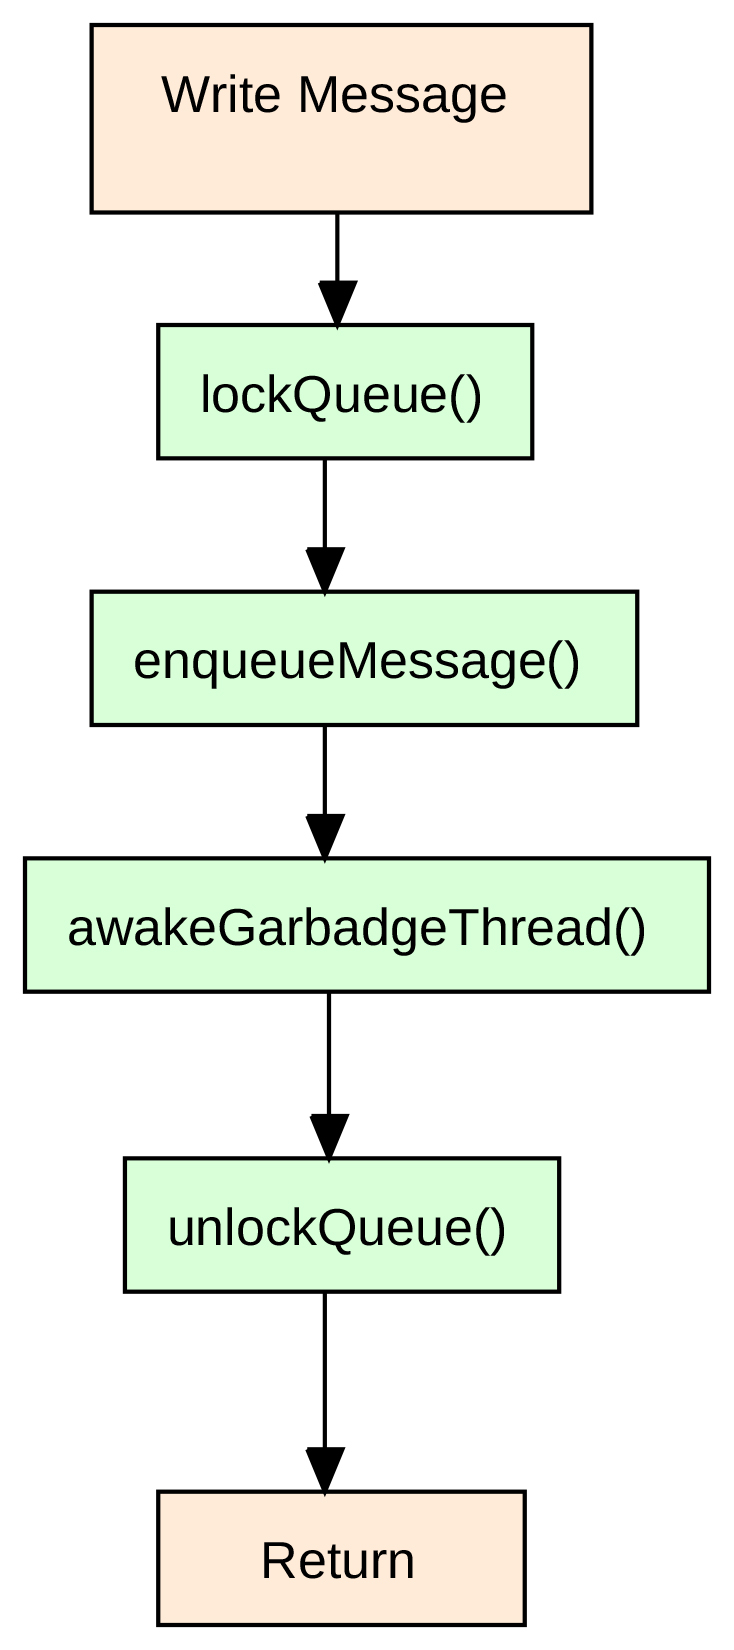
\includegraphics[width=12cm,height=7cm,keepaspectratio]{/home/giorgio/Scrivania/RelazioneIIW/miaParte/logger.jpg}
\end{center}



\end{frame}

\begin{frame}
\frametitle{Logger}
\framesubtitle{Scrittura del Garbage Thread}


\begin{center}
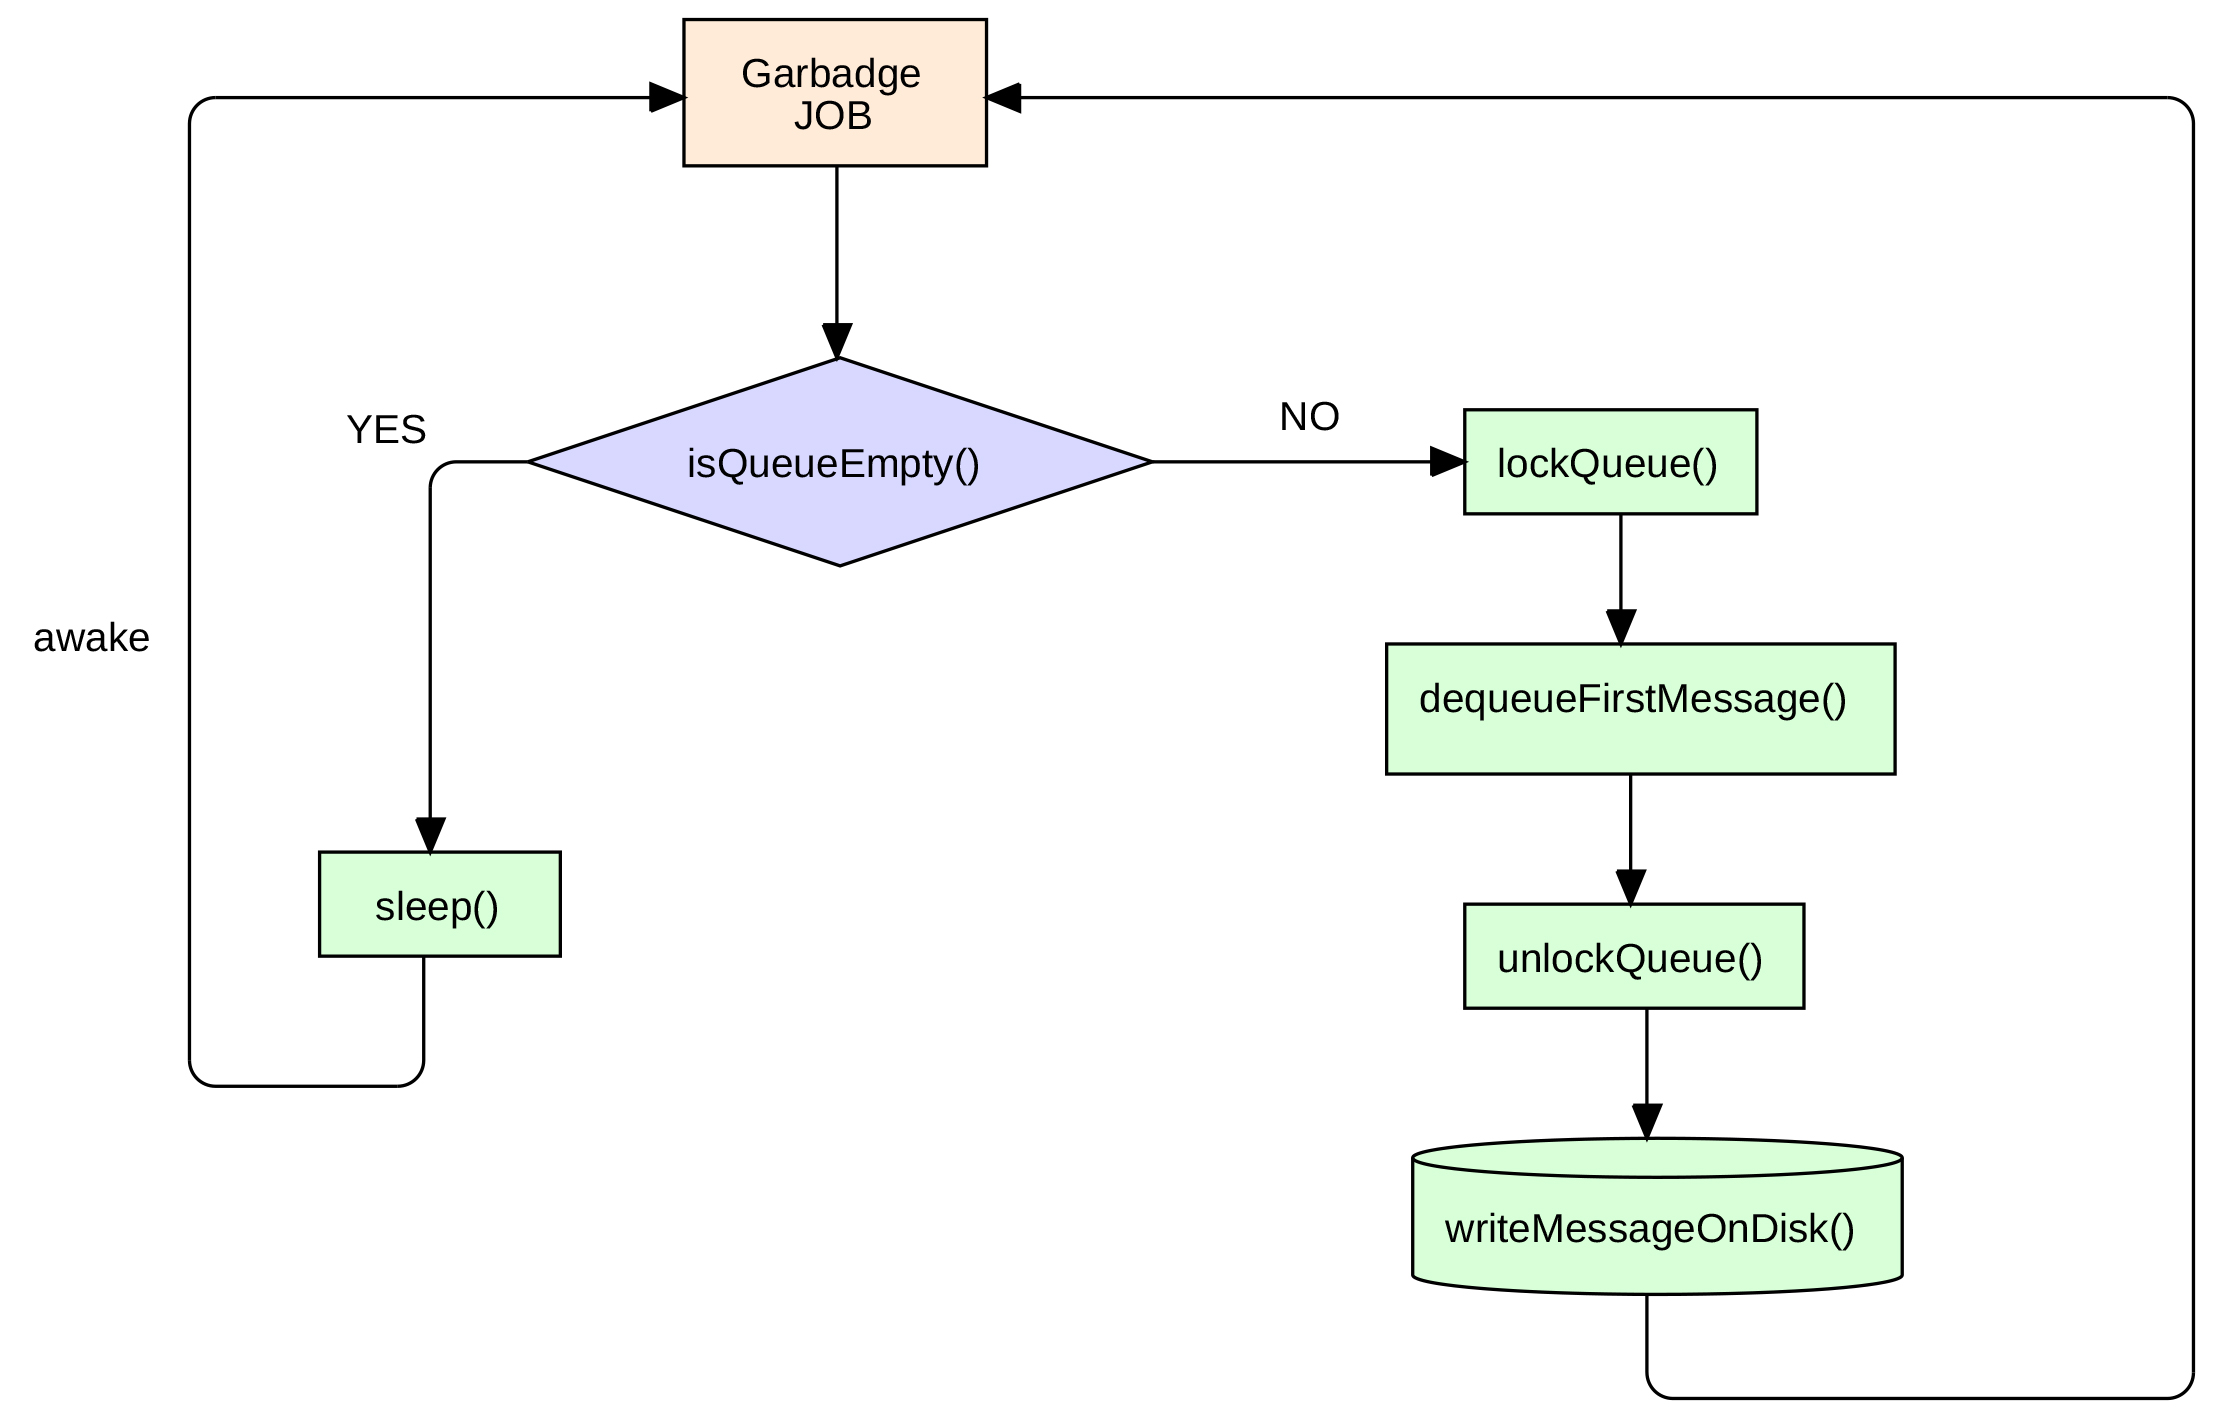
\includegraphics[width=11cm,height=8cm,keepaspectratio]{/home/giorgio/Scrivania/RelazioneIIW/miaParte/logger2.jpg}
\end{center}




\end{frame}
\frametitle{Logger}
\framesubtitle{Interfacce}
\begin{frame}[fragile]
\frametitle{Logger}
\framesubtitle{Interfacce}
\scriptsize
\begin{lstlisting}
struct logger * create_logger(char * pathLog, int log_lvl);
\end{lstlisting}
\normalsize

con:

\begin{itemize}
\item \texttt{pathLog}: percorso dove creare il file di log.
\item \texttt{log\_lvl}: livello del log.
\item restituisce un puntatore all'istanza logger creata.
\end{itemize}
\scriptsize
\begin{lstlisting}
void toLog(int type, struct logger * myLogger, char * buf, ...);
\end{lstlisting}
\normalsize

con:

\begin{itemize}
\item \texttt{type}: tipo di messaggio (Error, Warning o Info).
\item \texttt{myLogger}: puntatore all'istanza del logger.
\item \texttt{buf}: messaggio da scrivere (testo formattato, parametri illimitati).
\end{itemize}
\end{frame}


\begin{frame}
\frametitle{Performance e benchmarking}
\framesubtitle{Premesse}

\begin{itemize}
\item Prima di confrontare \textbf{Hideo} con \textbf{Apache} abbiamo condotto alcuni test preliminari
durante la fase di sviluppo per individuare un valore ottimale per il numero di
worker thread, successivamente individuato nel range di valori compreso tra 10 e
30 – di qui la decisione di utilizzare il valore 20.

\item I test, effettuati con \textbf{httperf}, hanno evidenziato come il server riesca a servire
senza rallentamenti, errori o warning fino 2305 connessioni al secondo.

\item Aumentando il numero di connessioni/secondo il server continua a funzionare,
tuttavia il degrado è significativo delle prestazioni (in particolare abbiamo
riportato valori decisamente discostanti nei tempi di risposta e nel tempo di
connessione medio ).
\end{itemize}
\end{frame}




\begin{frame}
\frametitle{Performance \& Benchmarking}
\framesubtitle{Test}

\begin{itemize}
\item Il plotting dei grafici è stato effettuato mediante la libreria Python \textbf{MatplotLib}.
\item In ascissa è riportato il valore del tasso di arrivo, misurato in richieste al secondo
(req/s); in ordinata, invece, è riportato il tempo corrispondente, misurato in
millisecondi(ms); in blu le prestazioni di Hideo, in rosso quelle di Apache2.
\end{itemize}

\end{frame}

\begin{frame}
\frametitle{Performance \& Benchmarking}
\framesubtitle{Average Connecion Time}
\begin{center}


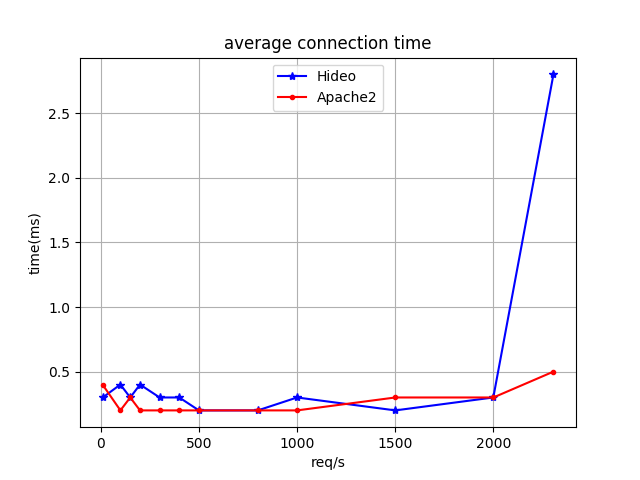
\includegraphics[width=10cm,height=10cm,keepaspectratio]{/home/giorgio/Scrivania/RelazioneIIW/miaParte/test_avg.png}
\end{center}
\end{frame}


\begin{frame}
\frametitle{Performance \& Benchmarking}
\framesubtitle{Average Connecion Time}
\begin{center}


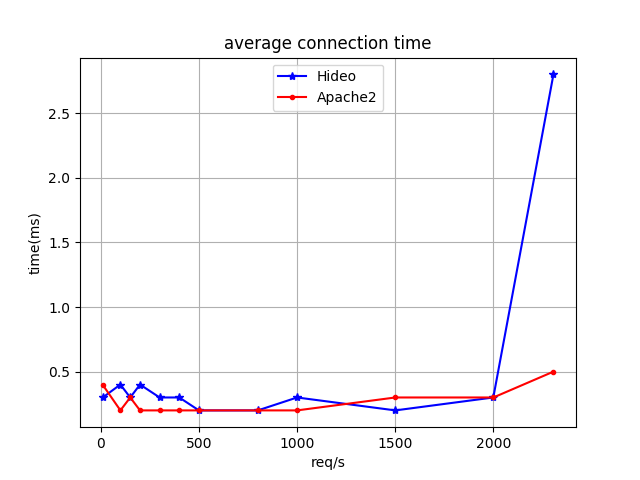
\includegraphics[width=10cm,height=10cm,keepaspectratio]{/home/giorgio/Scrivania/RelazioneIIW/miaParte/test_avg.png}
\end{center}
\end{frame}



\begin{frame}
\frametitle{Performance \& Benchmarking}
\framesubtitle{Minimum Connecion Time}
\begin{center}


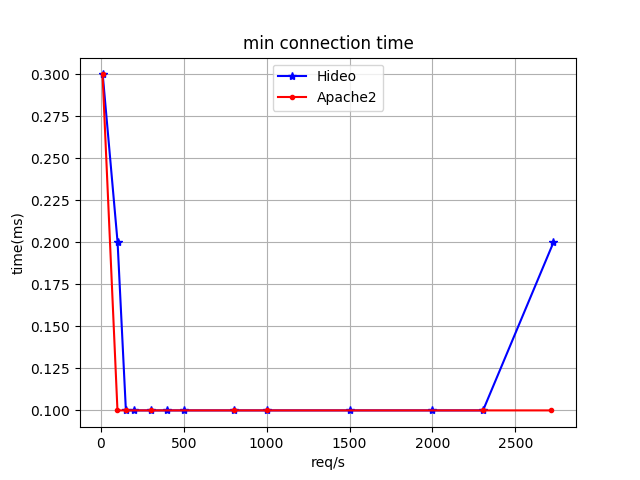
\includegraphics[width=10cm,height=10cm,keepaspectratio]{/home/giorgio/Scrivania/RelazioneIIW/miaParte/test_min.png}
\end{center}
\end{frame}




\begin{frame}
\frametitle{Performance \& Benchmarking}
\framesubtitle{Maximum Connecion Time}
\begin{center}


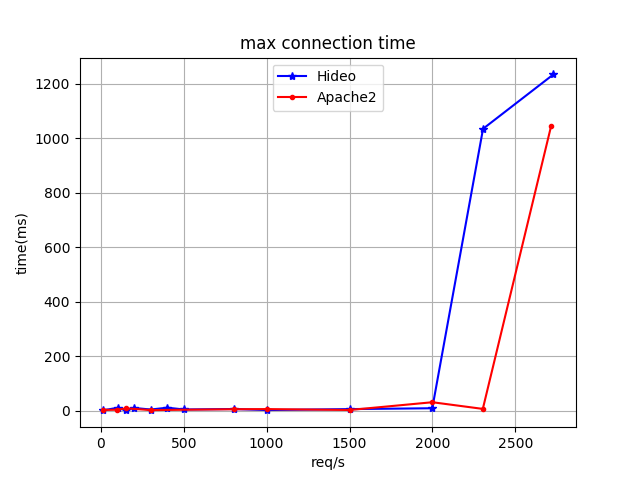
\includegraphics[width=10cm,height=10cm,keepaspectratio]{/home/giorgio/Scrivania/RelazioneIIW/miaParte/test_max.png}
\end{center}
\end{frame}




\begin{frame}
\frametitle{Performance \& Benchmarking}
\framesubtitle{Reply Time}
\begin{center}


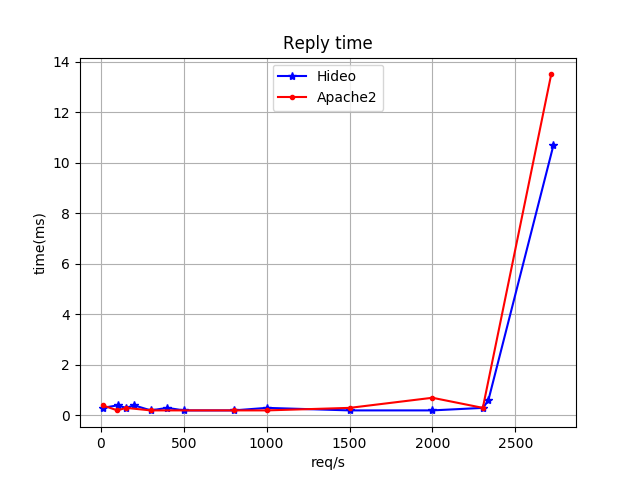
\includegraphics[width=10cm,height=10cm,keepaspectratio]{/home/giorgio/Scrivania/RelazioneIIW/miaParte/test_reply.png}
\end{center}
\end{frame}






\begin{frame}
\frametitle{Performance \& Benchmarking}
\framesubtitle{Analisi del Test}

\begin{itemize}
\item I test sono stati effettuati su macchina virtuale utilizzando la distribuzione \textit{GNU/Linux Xubuntu}.
\item Il motivo di tale decisione è dovuto
al fatto che \textbf{ScientiaMobile} ci ha fornito un pacchetto \textit{.deb} (quindi nativamente
supportata nelle distribuzioni Debian e derivate), oltre alla volontà di fornire un
ambiente pulito e minimale ad entrambi i server.
\item Dai risultati dei test, abbiamo constatato che i tempi di risposta fino ad un certo \textit{overhead} sono migliori di \textbf{Apache2}.
\end{itemize}
\end{frame}


\begin{frame}
\frametitle{Performance \& Benchmarking}
\framesubtitle{Analisi del Test}

\begin{itemize}
\item Una delle ipotesi per cui i tempi di risposta sono talvolta più stringenti è che
l’architettura di \textbf{Apache2} è molto più complessa (essendo multi-processo e multi-
thread) rispetto all’architettura di \textbf{Hideo}.
\item Questa complessità, tuttavia, si traduce in robustezza ed affidabilità nella risposta,
permettendo ad \textbf{Apache2} di mantenere prestazioni stabili molto oltre le 2000
connessioni simultanee.
\end{itemize}
\end{frame}




\begin{frame}
\frametitle{Utilizzo dell'Applicazione}
\framesubtitle{Prerequisiti}
Per la compilazione del Web Server sono necessari:
\begin{itemize}
\item Compilatore \textbf{GCC} versione $4+$.
\item Header C di sistema.
\item Pacchetto Header di WURFL.
\item Database di WURFL.
\end{itemize}








\end{frame}



\begin{frame}
\frametitle{Utilizzo dell'Applicazione}
\framesubtitle{Compilazione \& Configurazione}

\begin{itemize}
\item Per la compilazione del Web Server utilizzare i comandi \textit{make} e \textit{make clean}.

\item Per configurare il server modificare oppurtunamente il file \textit{server.cfg} attraverso i parametri:
\begin{itemize}
\medskip
\item \textbf{server}: Numero di porta sulla quale rimanere in ascolto.
\medskip
\item \textbf{threads}: Numero di thread del pool statico.
\medskip
\item \textbf{backlog}: Numero massimo di connessioni accettate in coda.
\medskip
\item \textbf{loglvl}: Tipologia di logging.
\end{itemize}
\end{itemize}

\end{frame}





\begin{frame}
\frametitle{Utilizzo dell'Applicazione}
\framesubtitle{Esecuzione}

\begin{itemize}
\item Una volta compilato e configurato, si può eseguire il server attraverso il comando \textit{./server}.
\item Il server sarà  disponibile all’indirizzo: \textbf{http://127.0.0.1:porta\_configurata}.
\item Il log del server sarà accodato al file \textit{server.log} (consultabile in tempo reale con il
comando \textit{tail -f server.log}).
\end{itemize}


\end{frame}



\end{document}
